\documentclass[table]{beamer}
\usepackage[utf8]{inputenc}
\usepackage{xcolor}
\usepackage{tcolorbox}
\usepackage{adjustbox}
\usepackage{multicol}
\usepackage{multirow}
\usepackage{eurosym}
\usepackage{amsmath}
\usepackage{ragged2e}
\usepackage[scaled]{helvet}
\usepackage{tikz}
\usepackage{eurosym}
\usepackage{enumerate}
\usetikzlibrary{spy,shapes,arrows,positioning,decorations.pathreplacing,matrix,calligraphy,calc}

\usepackage[style=british]{csquotes}

\def\signed #1{{\leavevmode\unskip\nobreak\hfil\penalty50\hskip1em
  \hbox{}\nobreak\hfill #1%
  \parfillskip=0pt \finalhyphendemerits=0 \endgraf}}

\newsavebox\mybox
\newenvironment{aquote}[1]
  {\savebox\mybox{#1}\begin{quote}\openautoquote\hspace*{-.7ex}}
  {\unskip\closeautoquote\vspace*{5mm}\signed{\usebox\mybox}\end{quote}}

\tikzset{hide on/.code={\only<#1>{\color{white}}}}
\definecolor{dark_green}{rgb}{0.0, 0.5, 0.0}

\pgfdeclarelayer{bg}    % declare background layer
\pgfsetlayers{bg,main}  % set the order of the layers (main is the standard layer)

\apptocmd{\frame}{}{\justifying}{}

\definecolor{iscal_color}{HTML}{641242} % ISCAL

\setbeamertemplate{footline}{
	\hspace{0.05\textwidth}
	\raisebox{3ex}{\insertshortauthor{}}\hfill
	\raisebox{3ex}{\insertframenumber{}/\inserttotalframenumber} \hfill
	{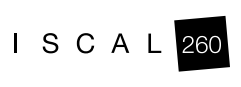
\includegraphics[height=0.08\textheight]{../visual material/logo.png}}
	\hspace{0.05\textwidth}
}

\tikzset{
  invisible/.style={opacity=0},
  visible on/.style={alt={#1{}{invisible}}},
  alt/.code args={<#1>#2#3}{%
    \alt<#1>{\pgfkeysalso{#2}}{\pgfkeysalso{#3}} % \pgfkeysalso doesn't change the path
  },
}

\title{Microeconomia}
\subtitle{Capitulo 4 : Monop\'olio v/s Concorr\^encia}
\author[]{}
\institute[ISCAL]{
\includegraphics[height=0.10\textheight]{../visual material/logo_eng_full.png}}
\date{Primavera 2020/2021}

\setbeamertemplate{navigation symbols}{}

\setbeamercolor{title}{fg = iscal_color}
\setbeamercolor{subtitle}{fg = iscal_color}
\setbeamercolor{frametitle}{fg = white, bg = iscal_color}

\hypersetup{linkcolor=iscal_color, colorlinks=true}

\AtBeginSection{\frame{\sectionpage}}
\renewcommand{\sectionname}{Parte}

\begin{document}

{
\setbeamertemplate{footline}{}
\begin{frame}
	\maketitle
\end{frame}
}

\begin{frame}{Conte\'udos}
  \tableofcontents
\end{frame}

\section{Monop\'olio}
\begin{frame}
	\frametitle{Monop\'olio}
	\begin{itemize}
		\setlength\itemsep{1.2em}
		\item<1-> Uma s\'o empresa produz um bem sem substitutos pr\'oximos
		\item<2-> H\'a barreiras \`a entrada no mercado:\onslide<3->{\footnote{\onslide<3->{1 e 2 s\~ao barreiras legais; 3 e 4 s\~ao barreiras estruturais ou naturais.}}}
		\begin{enumerate}
			\setlength\itemsep{1.1em}
			\item<3-> Acesso exclusivo a inputs/licen\c cas de explora\c c\~ao
			\item<3-> Patentes, regulamenta\c c\~oes
			\item<3-> Custos de entrada muito elevados
			\item<3-> Tecnologia com rendimentos crescentes \`a escala/economias de escala
		\end{enumerate}
	\end{itemize}
\end{frame}

\begin{frame}
	\frametitle{Maximiza\c c\~ao de lucro}
	A empresa pretende encontrar a quantidade a produzir tal que:\[\max\ \Pi = RT-CT\]
	\begin{columns}
		\begin{column}{0.47\textwidth}
			\begin{center}
				{\color{blue}Concorr\^encia perfeita}\par
				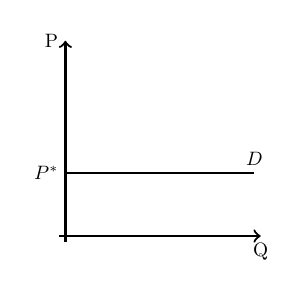
\begin{tikzpicture}[
					scale = 0.8,
					every node/.style = {scale = 0.7}
					]
					\draw[->,thick] (-0.1,0) -- (3.1,0)node[below]{Q};
					\draw[->,thick] (0,-0.1) -- (0,3.1)node[left]{P};

					\draw[thick] (0,1)node[left]{$P^*$} -- (3,1)node[above]{$D$};

				\end{tikzpicture}
				\[RT=P\times Q\]
			\end{center}
		\end{column}
		\begin{column}{0.47\textwidth}
			\begin{center}
				{\color{blue}Monop\'olio}\par
				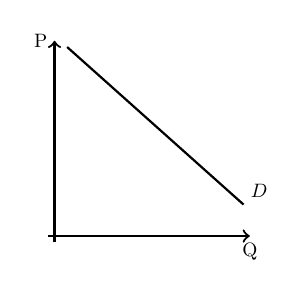
\begin{tikzpicture}[
					scale = 0.8,
					every node/.style = {scale = 0.7}
					]
					\draw[->,thick] (-0.1,0) -- (3.1,0)node[below]{Q};
					\draw[->,thick] (0,-0.1) -- (0,3.1)node[left]{P};

					\draw[thick] (0.2,3) -- (3,0.5)node[above right]{$D$};

				\end{tikzpicture}
				\[RT=P(Q)\times Q\]
			\end{center}
		\end{column}
	\end{columns}
\end{frame}

\begin{frame}
	\frametitle{Maximiza\c c\~ao do Lucro}
		Sendo \[\Pi = p(Q)\times Q - CV(Q) - CF\] 

		\pause

		A condi\c c\~ao de primeiro ordem (CPO) ser\'a: \pause
		\begin{align*}
			\frac{d\Pi}{dQ}=0 \Leftrightarrow \underbrace{p(Q)+Q\frac{dP(Q)}{dQ}}_{Rmg} - CV' = 0 \Leftrightarrow Rmg = Cmg > 0\
		\end{align*}\pause



		E a condi\c c\~ao de segundo ordem (CSO) ser\'a: \pause
		\begin{align*}
			\frac{d^2\Pi}{dQ^2} < 0 \Leftrightarrow \frac{dRmg}{dQ} < \frac{dCmg}{dQ}
		\end{align*}
\end{frame}

\begin{frame}
	\frametitle{Receita Marginal e Elasticidade da Procura}
	\begin{align*}
		\onslide<1->{Rmg &= Cmg > 0}\\
		\onslide<2->{Rmg &=P+Q\frac{dP}{dQ}}\\
		\onslide<3->{Rmg &=p\left(1+\frac{Q}{P}\frac{dP}{dQ}\right)}\\
		\onslide<4->{Rmg &=p\left(1+\frac{1}{\frac{P}{Q}\frac{dQ}{dP}}\right)}\\
		\onslide<5->{Rmg &= p\left(1+\frac{1}{\varepsilon_D}\right) = p \left(1-\frac{1}{|\varepsilon_D|}\right)}
	\end{align*}

\end{frame}

\begin{frame}
	\frametitle{Receita Marginal e Elasticidade da Procura}
	\begin{itemize}
		\item<1-> Sendo $\varepsilon_D=\frac{dQ}{dP}\frac{P}{Q}$ a elasticidade pre\c co da procura.
		\item<2-> A receita marginal s\'o ser\'a positiva na zona el\'astica da procura! Ent\~ao: 
		\item<3-> Se a procura \'e r\'igida, a $Rmg$ \'e negativa: se aumentar $Q$ colocada no mercado (por via de redu\c c\~ao de pre\c co), a Receita diminui (efeito pre\c co sobrep\~oe-se ao efeito quantidade), pelo que o monopolista nunca actuar\'a na zona r\'igida da procura...
	\end{itemize}

\end{frame}

\begin{frame}
	\frametitle{Receita Marginal e elasticidade}
	\begin{itemize}
		\setlength{\itemsep}{1.2em}
		\item<1-> NB: a receita do monopolista \'e igual \`a despesa de consumo...
		\item<2-> Revisitando o cap\'itulo 3A: qual a rela\c c\~ao entre altera\c c\~ao de pre\c co, despesa de consumo e elasticidade?
		\item<3-> Qual a implica\c c\~ao, sobre a despesa de consumo, do facto de o monopolista actuar apenas na zona el\'astica da procura?
	\end{itemize}
\end{frame}


\begin{frame}
	\frametitle{Elasticidade e Despesa de Consumo}
	\begin{columns}
		\begin{column}{0.47\textwidth}
			Generalizando os Resultados:
			\begin{align*}
				Despesa&=RT=P\times Q\\
				P&=\frac{a}{b}-\frac{1}{b}Q\\
				RT&=\left(\frac{a}{b}-\frac{1}{b}Q\right)\times Q\\
				&=\frac{a}{b}Q-\frac{1}{b}Q^2\\
				Rmg&=RT'=\frac{a}{b}-\frac{2}{b}Q\\
				Rmg&=0\Leftrightarrow Q=\frac{a}{2}
			\end{align*}
		\end{column}
		\begin{column}{0.47\textwidth}
			\begin{center}
				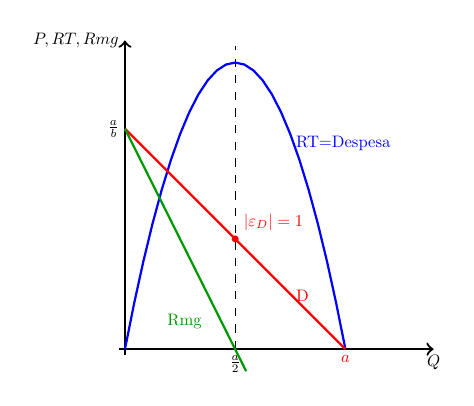
\begin{tikzpicture}[
					scale = 0.7,
					every node/.style = {scale = 0.6},
					declare function = {
						d(\x)=4-\x;
						rt(\x) = 1.3*(4-(\x-2)^2);
						rm(\x) = 4-(2)*\x;
					}]

					\draw[->,thick] (-0.1,0) -- (5.6,0)node[below]{$Q$};
					\draw[->,thick] (0,-0.1) -- (0,5.6)node[left]{$P,RT,Rmg$};
				
					\draw[dashed] (2,0)node[below]{$\frac{a}{2}$} -- (2,5.5);

					\draw[blue,thick,domain=0:4,variable=\x] plot (\x,{rt(\x)});
					\draw[blue] (3,3.5)node[above right]{RT=Despesa};

					\draw[red,thick,domain=0:4,variable=\x] plot (\x,{d(\x)}) node[below]{$a$};
					\draw[red] (3,0.75)node[above right]{D};	
					\draw[red] (2,2)node[circle,fill,inner sep=1.5,label=above right:{\(|\varepsilon_D|=1\)}]{};

					\draw[green!60!black,thick,domain=0:2.2,variable=\x] plot (\x,{rm(\x)});
					\draw[green!60!black] (1.5,0.5)node[left]{Rmg};
					\draw(0,{rm(0)}) node[left]{$\frac{a}{b}$};

				\end{tikzpicture}
			\end{center}
		\end{column}
	\end{columns}
\end{frame}

\begin{frame}
	\frametitle{Monop\'olio com procura linear}
	\begin{columns}
		\begin{column}{0.47\textwidth}
			\begin{center}
				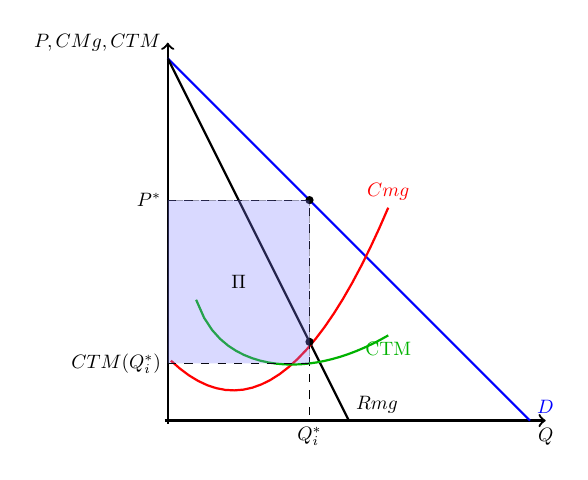
\begin{tikzpicture}[
					scale = 0.4,
					every node/.style = {scale =0.7},
					declare function = {
						d(\x) = 11.5-\x;
						rt(\x) = \x*d(\x);
						rmg(\x) = d(\x) - \x;
						cv(\x) = \x - (1/4)*\x^2 + (1/25)*\x^3;
						cf(\x) = 1;
						ct(\x) = cv(\x) + cf(\x);
						cmg(\x) = 1 - (2/4)*\x + (3/25)*\x^2;
						ctm(\x) = ct(\x)/\x;
					}
				]
					\def\p{4.5}

					\draw[->,thick] (-0.1,-0) -- (12,-0) node[below]{$Q$};
					\draw[->,thick] (0,-0.1) -- (0,12) node[left]{$P,CMg,CTM$};

					\onslide<1->{
						\draw[blue,thick,domain=0:11.5,variable=\x] plot (\x,{d(\x)})node[above right]{$D$};
						\draw[thick,domain=0:5.75,variable=\x] plot (\x,{rmg(\x)})node[above right]{$Rmg$};
					}

					\onslide<2->{
						\draw[red,thick,domain=0.1:7,variable=\x] plot (\x,{2*cmg(\x)-0})node[above]{$Cmg$};
					}

					\onslide<3->{
						\draw (\p,{rmg(\p)}) node[circle,fill,inner sep=1.5]{};
					}

					\onslide<4->{
						\draw[dashed] (0,{d(\p)})node[left]{$P^*$} -- (\p,{d(\p)})node[circle,fill,inner sep=1.5]{} -- (\p,0)node[below]{$Q_i^*$};		
					}

					\onslide<5->{
						\draw[green!70!black,thick,domain=0.9:7,variable=\x] plot (\x,{2*ctm(\x)-0})node[below]{CTM};
					}

					\onslide<6->{
						\draw[dashed] (0,{2*ctm(\p)})node[left]{$CTM(Q_i^*)$} -- (\p,{2*ctm(\p)});		
					}

					\onslide<7->{
						\draw[dashed,fill=blue!50!white,opacity=0.3] (0,{2*ctm(\p)}) -- (\p,{2*ctm(\p)}) --(\p,{d(\p)}) -- (0,{d(\p)}) -- (0,{2*ctm(\p)});
						\draw({\p/2},{(d(\p)+2*ctm(\p))/2}) node{$\Pi$};
					}	

				\end{tikzpicture}
			\end{center}
		\end{column}
		\begin{column}{0.47\textwidth}
			\begin{center}
				\onslide<2->{\(P=a-bQ\)}
				\onslide<3->{\(\Rightarrow RT=aQ-bQ^2\)}
				\onslide<4->{\(Rmg=RT'=a-2bQ\)}
				\vspace{0.25cm}
				\onslide<5->{
					\par \justify A curva da receita marginal tem o dobro do declive (em m\'odulo) da curva inversa da procura.\par
				}
				\onslide<7->{
					\[\Pi = RT-CT=Q(P-CTM)\]
				}

			\end{center}
		\end{column}
	\end{columns}
\end{frame}

\begin{frame}
	\frametitle{Excedente Econ\'omico em monop\'olio}
	\begin{center}
		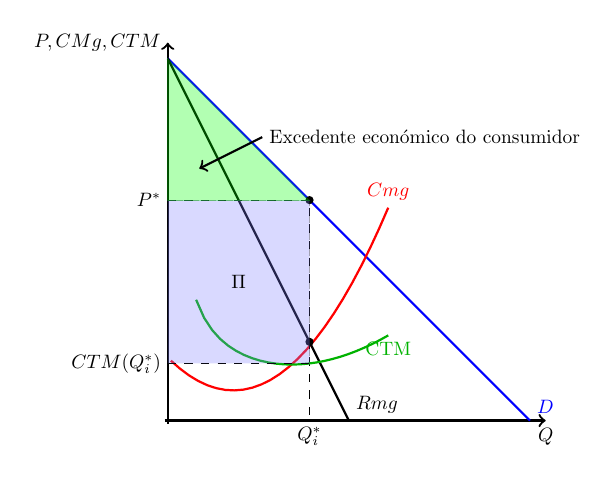
\begin{tikzpicture}[
			scale = 0.4,
			every node/.style = {scale =0.7},
			declare function = {
				d(\x) = 11.5-\x;
				rt(\x) = \x*d(\x);
				rmg(\x) = d(\x) - \x;
				cv(\x) = \x - (1/4)*\x^2 + (1/25)*\x^3;
				cf(\x) = 1;
				ct(\x) = cv(\x) + cf(\x);
				cmg(\x) = 1 - (2/4)*\x + (3/25)*\x^2;
				ctm(\x) = ct(\x)/\x;
			}
			]
			\def\p{4.5}

			\draw[->,thick] (-0.1,-0) -- (12,-0) node[below]{$Q$};
			\draw[->,thick] (0,-0.1) -- (0,12) node[left]{$P,CMg,CTM$};

			\draw[blue,thick,domain=0:11.5,variable=\x] plot (\x,{d(\x)})node[above right]{$D$};

			\draw[red,thick,domain=0.1:7,variable=\x] plot (\x,{2*cmg(\x)-0})node[above]{$Cmg$};
			\draw[thick,domain=0:5.75,variable=\x] plot (\x,{rmg(\x)})node[above right]{$Rmg$};

			\draw (\p,{rmg(\p)}) node[circle,fill,inner sep=1.5]{};

			\draw[dashed] (0,{d(\p)})node[left]{$P^*$} -- (\p,{d(\p)})node[circle,fill,inner sep=1.5]{} -- (\p,0)node[below]{$Q_i^*$};		

			\draw[green!70!black,thick,domain=0.9:7,variable=\x] plot (\x,{2*ctm(\x)-0})node[below]{CTM};

			\draw[dashed] (0,{2*ctm(\p)})node[left]{$CTM(Q_i^*)$} -- (\p,{2*ctm(\p)});		

			\draw[dashed,fill=blue!50!white,opacity=0.3] (0,{2*ctm(\p)}) -- (\p,{2*ctm(\p)}) --(\p,{d(\p)}) -- (0,{d(\p)}) -- (0,{2*ctm(\p)});
			\draw({\p/2},{(d(\p)+2*ctm(\p))/2}) node{$\Pi$};

			\draw[fill,green,opacity=0.3] (0,{d(0)}) -- (0,{d(\p)}) -- (\p,{d(\p)});

			\draw[thick,->] (3,9)node[right]{Excedente econ\'omico do consumidor} -- (1,8);

		\end{tikzpicture}
		\onslide<2->{\par E o excedente econ\'omico do produtor?}
	\end{center}	
\end{frame}

\begin{frame}
	\frametitle{Oferta em monop\'olio?}
	\begin{columns}
		\begin{column}{0.47\textwidth}
			\onslide<1->{
				Em concorr\^encia perfeita
				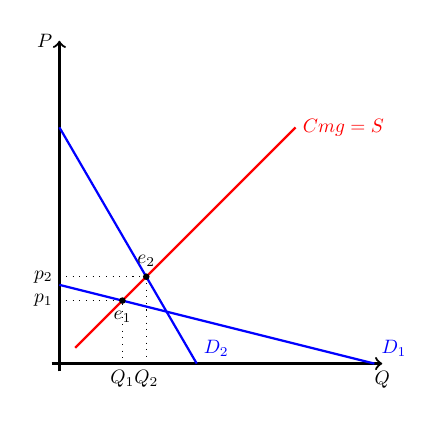
\begin{tikzpicture}[
						every node/.style = {scale = 0.7},
						declare function = {
							d1(\x) = 1-0.25*\x;
							d2(\x) = 3-1.72*\x;
							cmg(\x) = \x;
						}]

					\def\eqa{4/5}
					\def\eqb{3/2.72}

					\draw[thick,->](-0.1,0) --  (4.1,0)node[below]{$Q$};
					\draw[thick,->](0,-0.1) --  (0,4.1)node[left]{$P$};

					\draw[blue,thick,domain=0:4,variable=\x] plot (\x,{d1(\x)})node[above right]{$D_1$};
					\draw[blue,thick,domain=0:1.744,variable=\x] plot (\x,{d2(\x)})node[above right]{$D_2$};
					\draw[red,thick,domain=0.2:3,variable=\x] plot (\x,{cmg(\x)})node[right]{$Cmg=S$};

					\draw[dotted] (0,{cmg(\eqa)})node[left]{$p_1$} -- (\eqa,{cmg(\eqa)})node[circle,fill,inner sep=1.2,label=below:{$e_1$}]{} -- (\eqa,0)node[below]{$Q_1$};
					\draw[dotted] (0,{cmg(\eqb)})node[left]{$p_2$} -- (\eqb,{cmg(\eqb)})node[circle,fill,inner sep=1.2,label=above:{$e_2$}]{} -- (\eqb,0)node[below]{$Q_2$};

				\end{tikzpicture}
			}
		\end{column}
		\begin{column}{0.47\textwidth}
			\onslide<2->{
				Em monop\'olio
				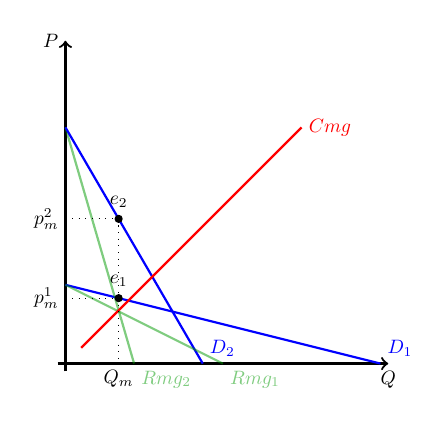
\begin{tikzpicture}[
						every node/.style = {scale = 0.7},
						declare function = {
							d1(\x) = 1-0.25*\x;
							rmg1(\x) = d1(\x) - 0.25*\x;							
							d2(\x) = 3-1.72*\x;
							rmg2(\x) = d2(\x) - 1.72*\x;
							cmg(\x) = \x;
						}]
	
					\def\eq{3/4.44}

					\draw[thick,->](-0.1,0) --  (4.1,0)node[below]{$Q$};
					\draw[thick,->](0,-0.1) --  (0,4.1)node[left]{$P$};

					\draw[blue,thick,domain=0:4,variable=\x] plot (\x,{d1(\x)})node[above right]{$D_1$};
					\draw[green!60!black,opacity=0.5,thick,domain=0:0.872,variable=\x] plot (\x,{rmg2(\x)})node[below right]{$Rmg_2$};

					\draw[blue,thick,domain=0:1.744,variable=\x] plot (\x,{d2(\x)})node[above right]{$D_2$};
					\draw[green!60!black,opacity=0.5,thick,domain=0:2,variable=\x] plot (\x,{rmg1(\x)})node[below right]{$Rmg_1$};
					
					\draw[red,thick,domain=0.2:3,variable=\x] plot (\x,{cmg(\x)})node[right]{$Cmg$};

					\draw[dotted] (0,{d1(\eq)})node[left]{$p_m^1$} -- (\eq,{d1(\eq)})node[circle,fill,inner sep=1.5,label=above:{$e_1$}]{} -- (\eq,0)node[below]{$Q_m$};

					\draw[dotted] (0,{d2(\eq)})node[left]{$p_m^2$} -- (\eq,{d2(\eq)})node[circle,fill,inner sep=1.5,label=above:{$e_2$}]{} -- (\eq,{d1(\eq)});

				\end{tikzpicture}
			}
		\end{column}
	\end{columns}
	\onslide<3->{
		\par No caso do monop\'olio \emph{\underline{podemos}} ter a mesma quantidade,\footnote{\onslide<3->{Poder n\~ao quer dizer que \'e um resultado garantido, s\'o poss\'ivel.}} e dois pre\c cos para duas procuras distintas!\par Assim ent\~ao, n\~ao podemos ter uma fun\c c\~ao oferta.
	}
\end{frame}

\begin{frame}
	\frametitle{Oferta em monop\'olio?}
	A rela\c c\~ao pre\c co quantidade depende da procura!, pelo que n\~ao existe uma oferta como a conhecemos.\par

	\vspace{1em}

	Assim, termos que calcular o excedente do produtor como vimos na defini\c c\~ao original, ou seja, como a receita menos os custos vari\'aveis.
\end{frame}

\begin{frame}
	\frametitle{Monopolista n\~ao produz}
	\begin{center}
		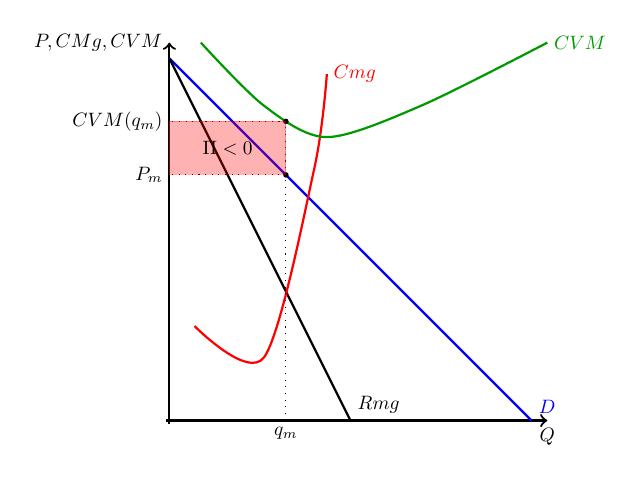
\begin{tikzpicture}[
			scale = 0.4,
			every node/.style = {scale =0.7},
			declare function = {
				d(\x) = 11.5-\x;
				rt(\x) = \x*d(\x);
				rmg(\x) = d(\x) - \x;
				cv(\x) = 4*(\x-4)- (1/4)*(\x-4)^2 + (1/25)*(\x-4)^3;
				cf(\x) = 1;
				ct(\x) = cv(\x) + cf(\x);
				cmg(\x) = 4 - (2/4)*(\x-4) + (3/25)*(\x-4)^2;
				ctm(\x) = ct(\x)/\x;
				cvm(\x) = cv(\x)/(\x-4);
			}
			]
			\def\p{4.5}

			\draw[->,thick] (-0.1,-0) -- (12,-0) node[below]{$Q$};
			\draw[->,thick] (0,-0.1) -- (0,12) node[left]{$P,CMg,CVM$};

			\draw[blue,thick,domain=0:11.5,variable=\x] plot (\x,{d(\x)})node[above right]{$D$};

			\draw[thick,domain=0:5.75,variable=\x] plot (\x,{rmg(\x)})node[above right]{$Rmg$};

			\draw[smooth,red,thick] plot coordinates {(0.8,3) (3,2) (4.6,8) (5,11)};
			\draw[smooth,green!60!black,thick] plot coordinates {(1,12) (3,10) (5,9) (8,10) (12,12)};

			\draw[red](5,11)node[right]{$Cmg$};
			\draw[green!60!black](12,12)node[right]{$CVM$};

			\def\qa{3.7}
			\def\vca{9.5}

			\onslide<2->{
				\draw[dotted] (\qa,0)node[below]{$q_m$} -- (\qa,\vca)node[circle,fill,inner sep=1]{} -- (0,\vca)node[left]{$CVM(q_m)$};
				\draw[dotted] (\qa,{d(\qa)})node[circle,fill,inner sep=1]{} -- (0,{d(\qa)})node[left]{$P_m$};
			}

			\onslide<3->{
				\draw[fill,red,opacity=0.3] (0,{d(\qa)}) -- (0,\vca) -- (\qa,\vca) -- (\qa,{d(\qa)});
				\draw[black] ({\qa/2},{(d(\qa)+\vca)/2}) node[black]{$\Pi<0$};
			}
		\end{tikzpicture}

		\onslide<4->{
			\par A procura seria demasiado pequena para os custos da ind\'ustria
		}

	\end{center}	
\end{frame}

\begin{frame}
	\frametitle{Monop\'olio vs. Concorr\^encia Perfeita}
	\begin{center}
		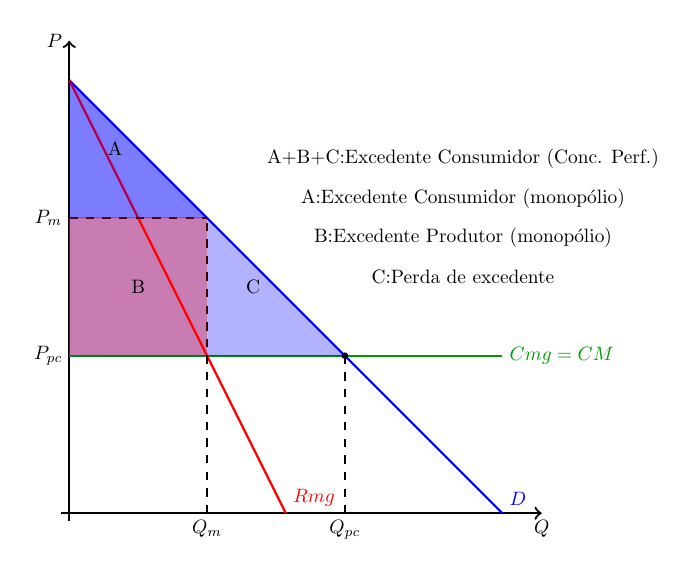
\begin{tikzpicture}[
			scale = 1,
			every node/.style = {scale =0.7},
			declare function = {
				d(\x) = 5.5-\x;
				rmg(\x) = 5.5-2*\x;
				cmg(\x) = 2;
			}
			]

			\def\eqcp{3.5}
			\def\eqcm{3.5/2}

			\draw[->,thick] (-0.1,-0) -- (6,-0) node[below]{$Q$};
			\draw[->,thick] (0,-0.1) -- (0,6) node[left]{$P$};

			\draw[thick,blue,domain=0:5.5,variable=\x] plot (\x,{d(\x)}) node[above right]{$D$};
			\draw[thick,green!60!black,domain=0:5.5,variable=\x] plot (\x,{cmg(\x)}) node[right]{$Cmg=CM$}; 

			\onslide<2->{
				\draw (0,{cmg(0)}) node[left]{$P_{pc}$};
				\draw[dashed,thick] (\eqcp,{d(\eqcp)})node[circle,fill,inner sep=1.2]{} -- (\eqcp,0) node[below]{$Q_{pc}$};
			}

			\onslide<3-6>{
				\draw[fill,blue,opacity=0.3] (0,{d(0)}) -- (\eqcp,{d(\eqcp)}) -- (0,{d(\eqcp)});
			}

			\onslide<4->{
				\draw[thick,red,domain=0:2.75,variable=\x] plot (\x,{rmg(\x)}) node[above right]{$Rmg$};
			}

			\onslide<5->{
				\draw[dashed,thick] (\eqcm,0)node[below]{$Q_m$} -- (\eqcm,{d(\eqcm)});
			}

			\onslide<6->{
				\draw[dashed,thick] (0,{d(\eqcm)})node[left]{$P_m$} -- (\eqcm,{d(\eqcm)});
			}

			\onslide<7->{
				\draw[fill,blue,opacity=0.3] (0,{d(0)}) -- (\eqcm,{d(\eqcm)}) -- (0,{d(\eqcm)});
				\draw[fill,red,opacity=0.3] (\eqcm,{d(\eqcm)}) -- (0,{d(\eqcm)}) -- (0,{d(\eqcp)}) -- (\eqcm,{d(\eqcp)});
			}

			\onslide<8->{
				\draw({\eqcm/3},{(d(\eqcm)+d(0))/2})node[]{A};
				\draw({\eqcm/2},{(d(\eqcm)+d(\eqcp))/2})node[]{B};
				\draw({\eqcm+(\eqcp-\eqcm)/3},{(d(\eqcm)+d(\eqcp))/2})node[]{C};
			}

			\onslide<9->{
				\draw(5,4.5) node[]{A+B+C:Excedente Consumidor (Conc. Perf.)};
				\draw(5,4) node[]{A:Excedente Consumidor (monop\'olio)};
				\draw(5,3.5) node[]{B:Excedente Produtor (monop\'olio)};
				\draw(5,3) node[]{C:Perda de excedente};
			}

		\end{tikzpicture}
	\end{center}
\end{frame}

\begin{frame}
	\frametitle{Nem sempre \'e vi\'avel um mercado concorrencial...}
	\begin{columns}
		\begin{column}{0.3\textwidth}
			\onslide<8->{\footnotesize
				\textbf{Economias de Escala:}
				limitam o n\'umero de empresas no mercado, constituindo ``barreiras naturais'' \`a entrada de empresas, dando \underline{poder de mercado} \`as empresas instaladas.. no limite, pode haver uma s\'o...
			}
		\end{column}
		\begin{column}{0.7\textwidth}
			\begin{center}
				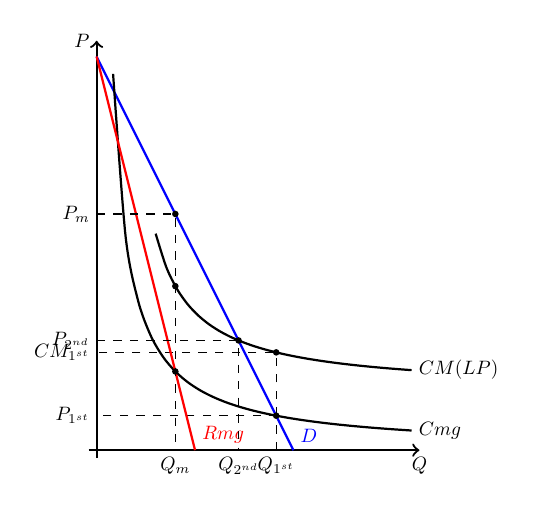
\begin{tikzpicture}[
					scale = 1,
					every node/.style = {scale =0.7},
					declare function = {
						d(\x) = 5-2*\x;
						rmg(\x) = 5-4*\x;
						cmg(\x) = 1/\x;
						cm(\x) = 1/(\x-0.25)+0.75;
					}
					]

					\def\qaa{2.2808} %1st best
					\def\qab{0.21922} % 1st worst
					\def\qba{1} % monop
					\def\qbb{1/4} %monop corte esq
					\def\qca{1.8031} % q of CMLP = D
					\def\qcb{0.57195} %
					

					\draw[->,thick] (-0.1,-0) -- (4.1,-0) node[below]{$Q$};
					\draw[->,thick] (0,-0.1) -- (0,5.2) node[left]{$P$};

					\onslide<2->{
						\draw[thick,blue,domain=0:2.5,variable=\x] plot (\x,{d(\x)}) node[above right]{$D$};
						\draw[thick,domain=(\qab-0.01):4,variable=\x,smooth] plot (\x,{cmg(\x)}) node[right]{$Cmg$};
					}

					\onslide<3-9>{
						\draw[dashed] (\qaa,0)node[below]{$Q_{1^{st}}$} -- (\qaa,{d(\qaa)}) node[circle,fill,inner sep=1.2]{} -- (0,{d(\qaa)}) node[left]{$P_{1^{st}}$};
					}

					\onslide<4->{
						\draw[thick,domain=0.75:4,variable=\x,smooth] plot (\x,{cm(\x)}) node[right]{$CM(LP)$};					
					}

					\onslide<5-9>{
						\draw[dashed] (\qaa,{d(\qaa)}) -- (\qaa,{cm(\qaa)})node[circle,fill,inner sep=1.2]{} -- (0,{cm(\qaa)})node[left]{$CM_{1^{st}}$};
					}

					\onslide<6->{
						\draw[thick,red,domain=0:1.25,variable=\x] plot (\x,{rmg(\x)}) node[above right]{$Rmg$};
					}

					\onslide<7-9>{
						\draw[dashed] (0,{d(\qba)})node[left]{$P_m$} -- (\qba,{d(\qba)})node[circle,fill,inner sep=1.2]{} -- (\qba,{cm(\qba)})node[circle,fill,inner sep=1.2]{} -- (\qba,{cmg(\qba)})node[circle,fill,inner sep=1.2]{} -- (\qba,0)node[below]{$Q_m$};
					}

					\onslide<10->{
						\draw[dashed] (0,{d(\qca)})node[left]{$P_{2^{nd}}$} -- (\qca,{d(\qca)})node[circle,fill,inner sep=1.2]{} -- (\qca,0)node[below]{$Q_{2^{nd}}$};
					}

				\end{tikzpicture}
			\end{center}
		\end{column}
	\end{columns}
	\onslide<9>{\footnotesize 1\textsuperscript{st} best ($P=Cmg$) n\~ao \'e vi\'avel na presen\c ca de Economias de Escala, j\'a que \'e um pre\c co que iria gerar um preju\'izo permanente.\par}
	\onslide<10>{\footnotesize E se pud\'essemos optar por um 2\textsuperscript{nd} best ($P=CM(LP)$)}
\end{frame}
\section{Monop\'olio Natural e Regula\c c\~ao}
\begin{frame}
	\frametitle{Monop\'olio Natural}
	Vamos imaginar a seguinte situa\c c\~ao:
	\begin{itemize}
		\setlength{\itemsep}{1.5em}
		\item Uma empresa, com custo marginal $c$ produz sozinha, otimamente $N$ unidades de um bem desejado pela sociedade
		\item Admita que a procura por esse bem seja $Q(p)$, e a procura inversa $P(q)$, ambas lineares.
	\end{itemize}
\end{frame}

\begin{frame}
	\frametitle{Monop\'olio Natural}
	\begin{center}
		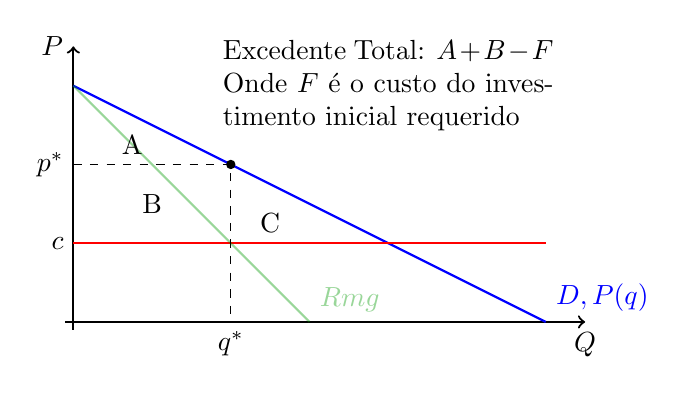
\begin{tikzpicture}[
			declare function = {
				d(\x) = 3-0.5*\x;
				rmg(\x) = 3-\x;
				c(\x) = 1;
			}]

			\def\q{2}

			\draw[->,thick] (-0.1,-0) -- (6.5,-0) node[below]{$Q$};
			\draw[->,thick] (0,-0.1) -- (0,3.5) node[left]{$P$};

			\draw[blue,thick,variable=\x,domain=0:6] plot (\x,{d(\x)}) node[above right]{$D,P(q)$};
			\draw[red,thick,variable=\x,domain=0:6] plot (\x,{c(\x)});
			\draw(0,{c(0)})node[left]{$c$};

			\onslide<2->{
				\draw[green!60!black,thick,variable=\x,domain=0:3,opacity=0.4] plot (\x,{rmg(\x)})node[above right]{$Rmg$};
			}

			\onslide<3->{
				\draw[dashed] (0,{d(\q)})node[left]{$p^*$} -- (\q,{d(\q)})node[circle,fill,inner sep=1.2]{} -- (\q,0)node[below]{$q^*$};
			}

			\onslide<4->{
				\draw(0.75,2.25) node[]{A};
				\draw(1,1.5) node[]{B};
				\draw(2.5,1.25) node[]{C};
			}

			\onslide<5->{
				\draw(4,3) node[]{\parbox{4.2cm}{Excedente Total: $A+B-F$ Onde $F$ \'e o custo do investimento inicial requerido}};
			}

		\end{tikzpicture}
	\end{center}
\end{frame}

\begin{frame}
	\frametitle{Monop\'olio Natural}
	Admita agora que entra uma segunda empresa, e por efeitos da concorr\^encia, o pre\c co desce ao n\'ivel do custo marginal:\[p^*=c\] Teremos ent\~ao a seguinte situa\c c\~ao:
\end{frame}

\begin{frame}
	\frametitle{Monop\'olio Natural}
	\begin{center}
		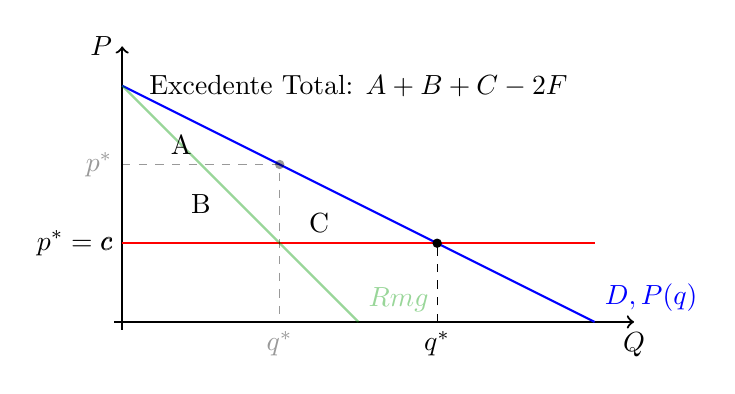
\begin{tikzpicture}[
			declare function = {
				d(\x) = 3-0.5*\x;
				rmg(\x) = 3-\x;
				c(\x) = 1;
			}]

			\def\q{2}
			\def\qe{4}

			\draw[->,thick] (-0.1,-0) -- (6.5,-0) node[below]{$Q$};
			\draw[->,thick] (0,-0.1) -- (0,3.5) node[left]{$P$};

			\draw[blue,thick,variable=\x,domain=0:6] plot (\x,{d(\x)}) node[above right]{$D,P(q)$};
			\draw[red,thick,variable=\x,domain=0:6] plot (\x,{c(\x)});
			\onslide<1>{
				\draw(0,{c(0)})node[left]{$c$};
			}

			\draw[green!60!black,thick,variable=\x,domain=0:3,opacity=0.4] plot (\x,{rmg(\x)})node[above right]{$Rmg$};

			\draw[dashed,opacity=0.4] (0,{d(\q)})node[left]{$p^*$} -- (\q,{d(\q)})node[circle,fill,inner sep=1.2]{} -- (\q,0)node[below]{$q^*$};

			\draw(0.75,2.25) node[]{A};
			\draw(1,1.5) node[]{B};
			\draw(2.5,1.25) node[]{C};

			\onslide<2->{
				\draw[dashed] (\qe,0)node[below]{$q^*$} -- (\qe,{d(\qe)})node[circle,fill,inner sep=1.2]{};
				\draw(0,{c(0)})node[left]{$p^*=c$};
			}

			\onslide<3->{
				\draw(3,3) node[]{Excedente Total: $A+B+C-2F$};
			}

		\end{tikzpicture}
	\end{center}
\end{frame}

\begin{frame}
	\frametitle{Monop\'olio Natural}
	Melhorou a situa\c c\~ao? \onslide<2->{Vejamos:
	\begin{align*}
		A+B+C-2F&>A+B-F\\
		C-F&>0\\
		C&>F
	\end{align*}
	}
	\onslide<3->{
	Ou seja, isto s\'o representa uma melhoria se os custos do investimento inicial necess\'ario foram menores que a \'area $C$, em outras palavras n\~ao \'e sempre o caso que acabar com um monop\'olio seja uma melhoria para o bem estar!
	}
\end{frame}

\begin{frame}
	\frametitle{Monop\'olio Natural}
	Economias de Escala em conjunto com uma procura de mercado pequena, podem reunir condi\c c\~oes para ter um monop\'olio natural, ou seja, apenas uma empresa \'e economicamente vi\'avel, porque consegue ter custos menores ao concentrar a produ\c c\`ao - subaditividade de custos na ind\'ustria.
\end{frame}

\begin{frame}
	\frametitle{Monop\'olio Natural}
	\begin{aquote}{Beaumol, AER 1977}
		A subaditividade da fun\c c\~ao de custos \'e condi\c c\`ao necess\'aria e suficiente para que um sector seja considerado monop\'olio natural.
	\end{aquote}
\end{frame}

\begin{frame}
	\frametitle{Monop\'olio Natural}
	A fun\c c\~ao de custos \'e \textbf{subaditiva} se o custo de produzir a quantidade $q$ com mais do que uma empresa \'e superior ao custo de produzir a mesma quantidade com s\'o uma empresa.
\end{frame}

\begin{frame}
	\frametitle{Monop\'olio Natural}
	Exemplo:
	\begin{itemize}
		\item A extens\~ao de Economias de Escala na produ\c c\~ao de energia el\'etrica \'e a mesma em qualquer parte do mundo, porque isso depende da tecnologia.\pause
		\item Num pa\'is pequeno (ex. Luxemburgo), a produ\c c\~ao de energia el\'etrica pode ser um monop\'olio natural, mas certamente n\~ao o \'e num pa\'is grande, com grande procura (ex. EUA), onde a produ\c c\~ao da quantidade procurada pode n\~ao ter custos m\'edios (na ind\'ustria) minimizados apenas com uma empresa.\pause
	\end{itemize}
	Em ambos os pa\'ises, a extens\~ao de Economias de Escala \'e semelhante, mas num caso haver\'a monop\'olio natural, noutro caso n\~ao (depende da dimens\~ao da Procura)
\end{frame}

\begin{frame}
	\frametitle{Qual o problema dos \emph{\underline{monop\'olios}}?}
	\begin{itemize}
		\item O equil\'ibrio de um mercado concorrencial maximiza o bem-estar conjunto das empresas e dos consumidores (Excedente econ\'omico), isto \'e:\pause
		\begin{itemize}
			\item As empresas escolhem a tecnologia otimamente, dados os pre\c cos dos fatores\pause
			\item Produzem o que os consumidores mais valorizam\pause
			\item Efici\^encia de Custos: output \'e produzido ao custo de oportunidade m\'inimo, o que exige efici\^encia t\'ecnica ao n\'ivel de cada empresa, mas tamb\'em que cada uma minimize os custos de oportunidade dos fatores.
		\end{itemize}
	\end{itemize}
\end{frame}

\begin{frame}
	\frametitle{Qual o problema dos \emph{\underline{monop\'olios}}?}
	Um monopolista, ao exercer o seu \textbf{poder de mercado}, afasta-se da situa\c c\~ao de equil\'ibrio concorrencial, o que gera uma perda de excedente econ\'omico.
\end{frame}

\begin{frame}
	\frametitle{E se houver um monop\'olio natural?}
	\'E prefer\'ivel haver um monop\'olio natural do que n\~ao existir mercado...\par\pause
	\vspace{0.4cm}
	Para evitar que a empresa ``abuse'' do consumidor, normalmente h\'a regula\c c\~ao de pre\c cos(pre\c co m\'aximo, por exemplo), j\'a que a situa\c c\~ao de monop\'olio natural normalmente surge em sectores ligados a infraestruturas que garantem servi\c cos p\'ublicos, onde n\~ao \'e eticamente aceit\'avel praticar-se pre\c cos muito altos.
\end{frame}

\begin{frame}
	\frametitle{Regula\c c\~ao de Pre\c cos}
	Uma solu\c c\~ao frequentemente usada \'e regular para que o monopolista cobre um pre\c co igual ao custo m\'edio de produ\c c\~ao, ficando na pr\' atica com lucro zero.\par
	
	\vspace{0.3cm}

	\'E a situa\c c\~ao de 2\textsuperscript{nd} Best, j\'a que n\~ao \'e vi\'avel ter $P=Cmg$ (1\textsuperscript{st} Best) - Pre\c cos de Ramsey.\par
	
	\vspace{0.3cm}

	O Estado, para conseguir que as empresas sigam esta pol\'itica, tem de pagar indemniza\c c\~oes compensat\'orias que teoricamente se deveriam aproximar do lucro que as empresas teriam se pudessem cobrar o pre\c co maximizador do lucro.
\end{frame}

\begin{frame}
	Problema?\pause\par
	\vspace{0.5cm}

	{\centering \Large As empresas perdem o incentivo a melhorar a produtividade e baixar os custos!
	}
\end{frame}

\begin{frame}
	Outra solu\c c\~ao implementada tem sido fixar pre\c cos m\'aximos e mante-los a\'i por algum per\'iodo de tempo.\pause\par
	\vspace{0.2cm}

	No come\c co, os \textbf{\underline{pre\c cos s\~ao fixados}} com base nos \textbf{\underline{custos de hoje}} da empresa, a modo da mesma ter lucros baixos ou nulos.\par
	\vspace{0.2cm}
	A empresa por outro lado, agora tem incentivos a melhorar a produtividade, pois assim poder\'a ter lucros pelos anos em que o pre\c co esteja fixo!
\end{frame}

\begin{frame}
	Problema?\pause\par

	\vspace{0.5cm}

	{\centering \Large O Governo tem incentivo a atualizar os pre\c cos depois do per\'iodo prometido para incluir as baixas nos custos, e assim a empresa pode fazer um menor esfor\c co em aumentar a produtividade, pois sabe que maiores baixas nos custos ir\~ao causar pre\c cos m\'aximos menores no pr\'oximo per\'iodo!.
	}
\end{frame}
\section{Discrimina\c c\~ao de pre\c cos}
\begin{frame}
	\frametitle{Poder de Mercado}
	Em geral, \'e a capacidade de uma empresa influenciar o pre\c co de venda do seu produto, bem como o pre\c copraticado pelas empresas concorrentes em mercados oligopolistas, atrav\'es de:
	\begin{itemize}
		\item Manipula\c c\~ao da vari\'avel estrat\'egica:
		\begin{itemize}
			\item Pre\c co
			\item Quantidade
		\end{itemize}
	\end{itemize}
\end{frame}

\begin{frame}
	\frametitle{Poder de Mercado}
	Fontes do poder de mercado:
	\begin{itemize}
		{\footnotesize
		\item Empresas instaladas em mercados com Barreiras \`a Entrada (barreiras naturais e barreiras legais);
		\item Empresas instaladas em nichos de mercado, explorando uma procura fiel ou fidelizada, enfrentando pouca concorr\^encia (bens sem substitutos);
		\item Diferencia\c c\~ao do prodto; cria\c c\~ao de procura fidelizada;
		\item Custos de transporte; custos de mudan\c ca; custos de busca de informa\c c\~ao
		}
	\end{itemize}
\end{frame}

\begin{frame}
	\frametitle{Discrimina\c c\~ao de Pre\c cos}
	Pr\'atica que consiste em fixar pre\c cos diferenttes para o mesmo produto, em fun\c c\~ao da quantidade comprada e/ou da disponibilidade a pagar do consumidor, em situa\c c\~oes em que as empresas t\^en \textbf{\underline{poder de mercado}}\par
	\vspace{0.5cm}
	A discrimina\c c\~ao ocorre quando uma empresa cobra pre\c cos diferentes:
	\begin{itemize}
		\item para cada unidade do bem, em fun\c c\~ao do pre\c co de reserva, ou seja, da disponibilidade a pagar, de cada consumidor (1\textsuperscript{\underline{o}} grau)
		\item para escal\~oes diferentes de consumo (2\textsuperscript{\underline{o}} grau)
		\item para grupos de consumidores ou mercados distintos (3\textsuperscript{\underline{o}} grau)
	\end{itemize}
\end{frame}

\begin{frame}
	\frametitle{Cond\c c\~oes para que a discrimina\c c\~ao de pre\c cos seja vi\'avel}
	\begin{itemize}
		\setlength{\itemsep}{1.2em}
		\item O vendedor tem que ser capaz de identificar os diferentes consumidores
		\item N\~ao pode existir revenda (comprar mais barato para vender mais caro)
	\end{itemize}
\end{frame}

\begin{frame}
	\frametitle{A Discrimina\c c\~ao Perfeita (1\textsuperscript{\underline{o}} Grau)}
	\begin{itemize}
		\setlength{\itemsep}{1.5em}
		\item O monopolista cobra o pre\c co mais alto que cada consumidor est\'a disposto a pagar (pre\c co de reserva).
		\item A Procura coincide com a curva da receita marginal. O excedente do consumidor anula-se...
		\item A produ\c c\~ao total \'e igual \`a que se obt\'em em concorr\^encia perfeita, vejamos...
	\end{itemize}
\end{frame}

\begin{frame}
	\frametitle{A Discrimina\c c\~ao Perfeita (1\textsuperscript{\underline{o}} Grau)}
	Caso em que o $Cmg$ \'e constante
	\begin{columns}
		\begin{column}{0.47\textwidth}
			\begin{center}
				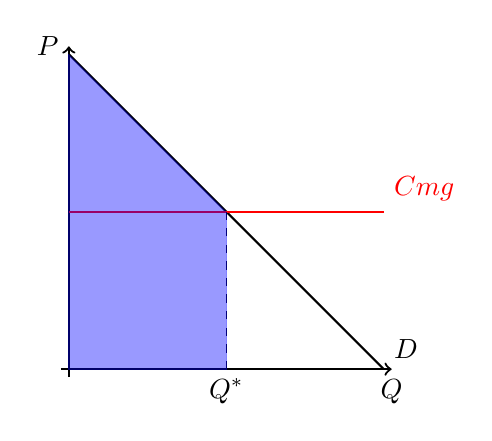
\begin{tikzpicture}[
					declare function = {
						d(\x) = 4-\x;
						cmg(\x) = 2;
					}]
					\draw[thick,->] (-0.1,0) -- (4.1,0)node[below]{$Q$};
					\draw[thick,->] (0,-0.1) -- (0,4.1)node[left]{$P$};

					\draw[domain=0:4,variable=\x,thick] plot (\x,{d(\x)})node[above right]{$D$};
					\draw[domain=0:4,variable=\x,red,thick] plot (\x,{cmg(\x)})node[above right]{$Cmg$};

					\draw[dashed] (2,0)node[below]{$Q^*$} -- (2,{d(2)});

					\onslide<2->{
						\draw[fill,blue,opacity=0.4] (0,4) -- (0,0) -- (2,0) -- (2,2);
					}
				\end{tikzpicture}
			\end{center}
		\end{column}
		\begin{column}{0.47\textwidth}
			\begin{itemize}
				{\footnotesize
				\item $Rmg=P$,  j\'a que o produtor cobra o pre\c co de reserva, i.e., o m\'aximo que o consumidor est\'a disposto a pagar...
				\item Ent\~ao a quantidade \'optima ocorre quando $Cmg=P$
				\item Do ponto de vista de efici\^encia, esta situa\c c\~ao \'e id\^entica \`a de concorr\^encia perfeita, mas do ponto de vista de quidade \'e contr\'aria... porqu\^e?
				\item A \'area sobreada coincide com a receita do produtor. O excedente que seria do consumidor \'e, agora, do produtor...
				}
			\end{itemize}
		\end{column}
	\end{columns}
\end{frame}

\begin{frame}
	\frametitle{A Discrimina\c de pre\c cos de 2\textsuperscript{\underline{o}} Grau}
	\begin{itemize}
		\setlength{\itemsep}{1.5em}
		\item O produtor cobra pre\c cos diferentes para escal\~oes diferentes de consumo de um bem ou servi\c co (venda por \emph{blocos})
		\item Aplica-se essencialmente quando os custos marginais s\~ao constantes
		\item \'E o caso dos descontos de quantidade...
	\end{itemize}
\end{frame}

\begin{frame}
	\frametitle{A discrimina\c do 3\textsuperscript{\underline{o}} Grau}
	\begin{itemize}
		\setlength{\itemsep}{1.5em}
		\item O produtor cobra pre\c cos diferentes a consumidores diferentes (ou em mercados diferentes). Realiza, deste modo, uma segmenta\c c\~ao do mercado aproveeitando a exist\^encia de pre\c cos de reserva distintos.
		\item Exemplos:
		\begin{itemize}
			\item descontos a estudantes ou a idosos
			\item produtos vendidos em mercados diferentes ou segmentos de mercado diferentes
		\end{itemize}
		\item \emph{O objectivo \'e sempre o mesmo: transformar excedente de consumidor em receita...\'e uma forma de exerc\'icio de poder de mercado}
	\end{itemize}
\end{frame}
\section{Defesa da concorr\^encia}
\begin{frame}
	\frametitle{Defesa de Concorr\^encia: O que \'e?}
	\begin{aquote}{Massimo Motta}
		Conjunto de pol\'iticas e leis que garantem que a concorr\^encia no mercado n\~ao \'e restringida de forma a que se reduza o bem-estar social.
	\end{aquote}
	
	\vspace{0.5cm}

	\begin{itemize}
		\item O bem-estar social \'e o objectivo a atingir com a pol\'itica de concorr\^encia.
		\item Tem particular relev\^ancia em mercados onde as empresas t\^em poder de mercado e onde a concorr\^encia \'e vi\'avel!
	\end{itemize}
\end{frame}

\begin{frame}
	\frametitle{Por que raz\~ao \'e necess\'aria a Defesa da Concorr\^encia?}
	Mesmo em mercados que funcionariam concorrencialmente, as for\c cas de mercado poderiam n\~ao levar ao resultado eficiente porque:
	\begin{itemize}
		\item As empresas podem comportar-se estrategicamente
		\item Podem criar ou fortalecer posi\c c\~oes dominantes atrav\'es de opera\c c\~oes de concentra\c c\~ao
		\item Podem efetuar ac\c c\~oes que aumentem os lucros e reduzam o bem-estar social: conluio, comportamento predat\'orio
	\end{itemize}
\end{frame}

\begin{frame}
	\frametitle{Conluio}
	\begin{itemize}
		\item Comportamento concertado de empresas (carteliza\c c\~ao, conluio) corresponde ao estabelecimento, por via de um acordo, de:
		\begin{itemize}
			\item Pre\c cos superiores a um padr\~ao;
			\item Quotas de mercado;
			\item Divis\~ao de mercados
		\end{itemize}
		\item Este acordo pode ser expl\'icito ou impl\'icito(conluio t\'acito)
		\item O acordo permite \`as empresas envolvidas usufruir de poder de mercado qeu de outra forma n\~ao teriam.
	\end{itemize}
\end{frame}

\begin{frame}
	\frametitle{Detec\c c\~ao de acordos entre empresas}
	\begin{itemize}
		\item A dissuas\~ao depende do n\'ivel das penas e o conluio \'e sujeito a pesadas penas: multas, pagamento de indemniza\c c\~oes e nos EUA at\'e penas de pris\~ao. Mas o valor esperado da pena \'e respetivo valor vezes a probabilidade de detec\c c\~ao...
		\item A melhor pol\'itica face ao conluio \'e criar mecanismos que tornem dif\'icil a emerg\^encia ou a sustentabilidade do acordo
	\end{itemize}
\end{frame}

\begin{frame}
	\frametitle{Abusos de Posi\c c\~ao Dominante}
	\begin{itemize}
		\item Um comportamento \'e predat\'orio se tem como objetivo proteger ou aumentar o poder de mercado de uma empresa dominante, atrav\'es da exclus\~ao ou elimina\c c\~ao de concorrentes por raz\~oes que n\~ao a sua efici\^encia.
		\item A exclus\~ao pode fazer-se atrav\'es da pr\'atica de pre\c cos baixos pela empresa dominante que baixem as receitas dos concorrentes.
	\end{itemize}
\end{frame}

\begin{frame}
	\frametitle{Pr\'aticas Predat\'orias}
	\begin{itemize}
		\item Direitos exclusivos de acesso a inputs
		\item Recusa de acesso a infra-estruturas essenciais
		\item Dumping
	\end{itemize}
\end{frame}

\begin{frame}
	\frametitle{Autoridade da Concorr\^encia-Lei da Concorr\^encia}
	\footnotesize{Lei 18/3004, Artigo 4\textsuperscript{\underline{o}}, Pr\'aticas proibidas:}
	
	\begin{enumerate}
		{\scriptsize
		\item S\~ao proibidos os acordos entre empresas, as decis\~oes de associa\c c\~oes de empresas e as pr\'aticas concertadas entre empresas, qualquer que seja a forma que revistam, que tenham por objeto ou como efeito impedir, falsear ou restringir de forma sens\'ivel a concorr\^encia no todo ou em parte do mercado nacional, nomeadamente os que se traduzam em:
		\begin{enumerate}[a)]
			{\scriptsize
			\item Fixar, de forma direta ou indireta, os pre\c cos de compra ou de venda ou interferir na sua determina\c c\~ao pelo livre jogo do mercado, induzindo, artificialmente, quer a sua alta quer a sua baixa;
			\item Fixar, de forma direta ou indireta, outras condi\c c\~oes de transac\c c\~ao efetuadas no mesmo ou em diferentes est\'adios do processo econ\'omico;
			\item Limitar ou controlar a produ\c c\~ao, a distribui\c c\~ao, o desenvolvimento t\'ecnico ou os investimentos;
			\item Repartir os mercados ou as fontes de abastecimento;
			\item Aplicar, de forma sistem\'atica ou ocasional, condi\c c\~oes discrminat\'orias de pre\c co ou outras relativamente a presta\c c\~oes equivalentes;
			\item Recusar, direta ou indiretamente, a compra ou venda de bens e a presta\c c\~oe de servi\c cos;
			\item Subordinar a celebra\c c\~ao de contratos \`a aceita\c c\~ao de obriga\c c\~oes suplementares que, pela sua natureza, ou segundo os usos comerciais, n\~ao tenham liga\c c\~ao com o objeto desses contratos.
			}
		\end{enumerate}
		}
	\end{enumerate}
\end{frame}

\end{document}